% GENERATED by `python -m bench.figures --write` from
% bench/results/counter_sweep.json. Do not edit: `--check` runs in CI
% and fails if this file and the committed runs disagree.
\begin{figure}[t]
\centering
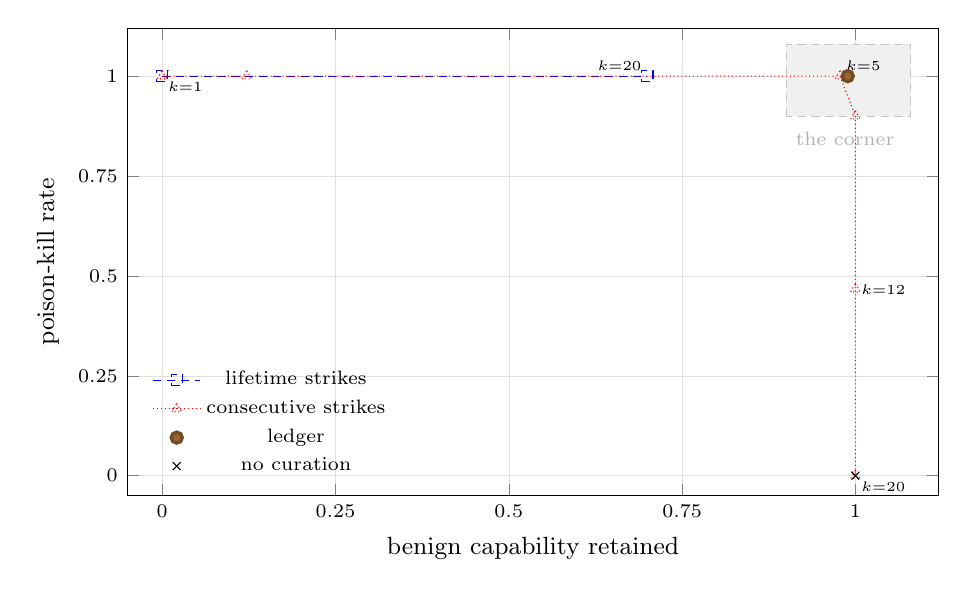
\begin{tikzpicture}
  \begin{axis}[
    width=0.98\columnwidth, height=0.62\columnwidth,
    xlabel={benign capability retained}, ylabel={poison-kill rate},
    xmin=-0.05, xmax=1.12, ymin=-0.05, ymax=1.12,
    xtick={0,0.25,0.5,0.75,1}, ytick={0,0.25,0.5,0.75,1},
    tick label style={font=\scriptsize},
    label style={font=\small},
    grid=major, grid style={very thin, gray!25},
    legend style={font=\scriptsize, at={(0.02,0.02)}, anchor=south west, draw=none, fill=none},
  ]
      \draw[fill=gray!12, draw=gray!45, densely dashed]
        (axis cs:0.9,0.9) rectangle (axis cs:1.08,1.08);
      \node[font=\scriptsize, gray!60, anchor=north east] at
        (axis cs:1.07,0.885) {the corner};
      \addplot+[mark=square, densely dashed] coordinates {(0.0000,1.0000) (0.0000,1.0000) (0.0000,1.0000) (0.0000,1.0000) (0.0000,1.0000) (0.0000,1.0000) (0.7000,1.0000)};
      \addlegendentry{lifetime strikes}
      \node[font=\tiny, anchor=north west, inner sep=2pt] at (axis cs:0.0000,1.0000) {$k{=}1$};
      \node[font=\tiny, anchor=south east, inner sep=2pt] at (axis cs:0.7000,1.0000) {$k{=}20$};
      \addplot+[mark=triangle, densely dotted] coordinates {(0.0000,1.0000) (0.0000,1.0000) (0.1222,1.0000) (0.9778,1.0000) (1.0000,0.9000) (1.0000,0.4667) (1.0000,0.0000)};
      \addlegendentry{consecutive strikes}
      \node[font=\tiny, anchor=south west, inner sep=2pt] at (axis cs:0.9778,1.0000) {$k{=}5$};
      \node[font=\tiny, anchor=west, inner sep=2pt] at (axis cs:1.0000,0.4667) {$k{=}12$};
      \node[font=\tiny, anchor=north west, inner sep=2pt] at (axis cs:1.0000,0.0000) {$k{=}20$};
      \addplot+[only marks, mark=*, very thick] coordinates {(0.9889,1.0000)};
      \addlegendentry{ledger}
      \addplot+[only marks, mark=x] coordinates {(1.0000,0.0000)};
      \addlegendentry{no curation}
  \end{axis}
\end{tikzpicture}
\caption{The strike counter's dial at $b{=}2$, 30 seeds, plotted in the
plane it has to win in. A defence must hold both axes, so the target is
the shaded corner. Raising $k$ walks each counter rightwards --- it keeps
more benign memory --- but the two shapes arrive differently. The
consecutive path enters the corner at $k{=}5$ and leaves it again by
$k{=}12$, falling down the right edge toward no curation at all: that is
the refutation of our pre-registered prediction, and it is why the paper
no longer claims the corner is the ledger's alone. The lifetime path
never enters it at any $k$ we tested, staying pinned to the top edge
because poison keeps earning lifetime blame however high the threshold.
The ledger sits in the corner untuned. Generated from committed per-seed
data by \texttt{bench/figures.py}; CI fails if the two disagree.}
\label{fig:countersweep}
\end{figure}
